\documentclass{article}
\usepackage{graphicx}
\begin{document}

\textbf{Editors}

\textsc{Reviewer 1}

\underline{State key points and conclusions at the beginning}:

\textbf{Reviewer}: \textit{In terms of its overall organization, your paper is (probably, necessarily) complicated. For me, the discussion/conclusion (Section 5) is much more clear and powerfully written than is the abstract and Introduction (Section 1). As you think about improving the paper, I hope you will find ways to assert the main Section 5 points crisply at the beginning of the paper.} 

\textbf{Response}: 

\underline{Add distinction between Bonacich and CA to the highlights}:

\textbf{Reviewer}: \textit{(For example, I would like to see a ``Highlights" bullet point that says that Bonacich centrality is useful for revealing the position of the nodes in a center-periphery pattern, to the extent one exists, whereas CA is useful for revealing the presence of different groups or communities in the data, to the extent that the dual network is not homogeneous.)}

\textbf{Response}: Thanks for this suggestion. I have now included a relevant highlight bulletpoint noting the relevant analytic contrast of Bonacich versus CA.

\underline{Data errors in the Southern Women two-mode matrix}:

\textbf{Reviewer}: \textit{Importantly, there are 4 errors in the matrix (``Southern Women data") that you analyze. For this dataset, you (in the note to Table 1) cite Doreian et al (2004, Table 4). Among the attendees at Event E4, you show Frances, Eleanor, and Ruth. However they did not attend this event. You also show Nora as absent from Event E8; however, Nora attended E8. These four errors are discrepant in comparison to your cited source (Doreian et al, 2004, Table 4), and they are discrepant as well in comparison to the original source (Davis, Gardener, and Gardener, 1941, p. 141, which has events in the same order as in your Table 1, and a slightly different order of women; this table is reproduced in Freeman, 2003, p. 42).}

\begin{figure}[h!]
    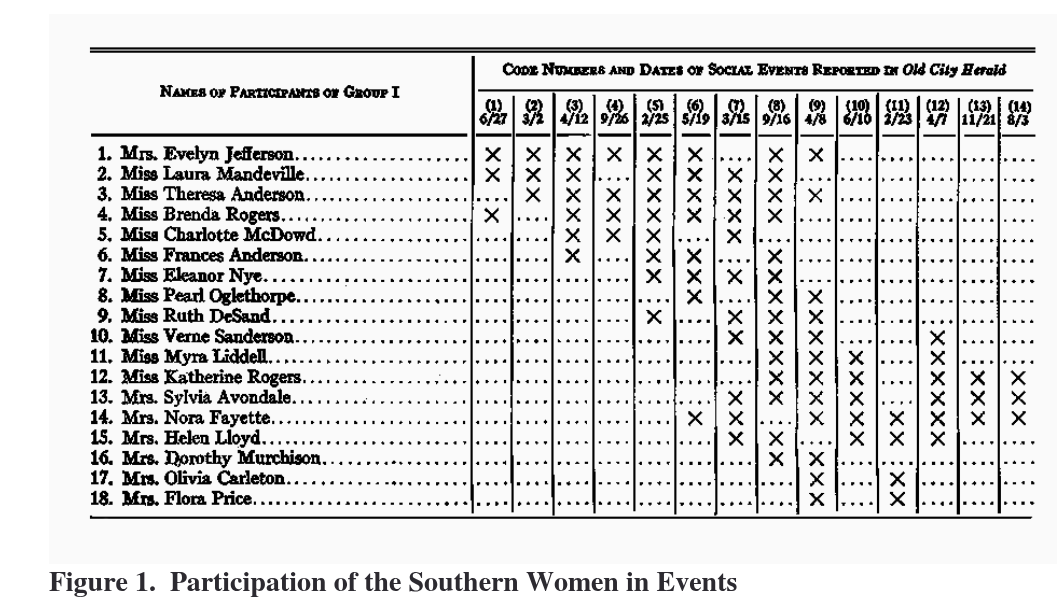
\includegraphics[width=1.0\textwidth]{Reviews and Response/sw-original.png}
\end{figure}

\textbf{Response}: Thanks for calling attention to this---rather embarrassing---error; it's definitely a cautionary tale against manually copying data. I have corrected the data, and as you can see in the analysis file included as supplementary material, I now extract the Southern Women data directly from the \texttt{networkdata} package. My table now matches those in the references you mentioned exactly. Note, however, that while you are correct that Frances, Eleanor, and Ruth did not attend E4, Nora did not attend E8, at least according to the published tables in Doreian et al (2004), Kovacs (2010), and the Figure 1 from Freeman (2003), shown above; in these papers, as you can see, Nora's event set is \{E6, E7, E9, E10, E11, E12, E13, E14\}. I think the confusion comes from the fact that Freeman used a non-chronological order of events (as is evident from the date labels in the figure) that emphasizes the group structure of the women. This non-chronological ordering leads to a different labeling of events than when events are arranged in chronological order; this is the ordering of events used by Doreian et al. 2004 and Kovacs (2010). In this event labeling, Nora does not attend E8 (the event that took place on 9/16.) However, note that this is obviously \textit{not} the ordering of events in the original Breiger (1974)---nor for that matter the earlier Doreian (1979) piece in \textit{Social Networks} that used Q-Analysis. In this \textit{chronological} labeling of events, Nora does attend ``E8" (the event that took place on 5/19), as evident in Breiger (1974, p. 186, fig. 2a). In any case, to forestall any confusion, and given that the in the \texttt{networkdata} package, the \texttt{igraph} object containing the Southern Women data come ordered using the Freeman (2003) ordering, I'm sticking to the non-chronological event labeling. I now include a brief discussion in the paper clarifying this issue. 

\underline{Appropriateness of the term ``reflective centrality''}:

\textbf{Reviewer}: \textit{I have some resistance to your term "reflective centrality" (Section 2 title) to characterize the scores of the respective modes - precisely because, as you importantly show, in the limit the reflective scores are first dimensions of a CA, and (as you also importantly emphasize) the first CA dimension is about finding groups, not about ordering nodes. Hidalgo and Hausmann (2009) do not use the term "centrality" for the reflective scores they define and compute. I wonder whether ``reflective scores" might be a better term; I'm not sure, and simply ask you to think about it.}

\textbf{Response}:

\underline{Differences between odd and even iterations}:

\textbf{Reviewer}: \textit{What complicates things, as you know, is the difference between odd and even iterations of the reflective algorithm (see your comments in the first paragraph on p. 4, as well as comments of H \& H). One point you might consider adding is that, for the first even iterations (iterations 2, 4, 6, 8, and 10), the magnitude (absolute value) of the correlation of reflected scores with Bonacich centrality (for persons, and for groups) tends to increase with subsequent iterations (and, in the limit, is .682 for persons by iteration 40 for persons), whereas, for the first odd iterations (iterations 3, 5, 7, 9, 11), the magnitude of the correlation decreases (toward a limiting value, once again, of .682 by iteration 41). Can you relate this to the differences between odd and even iterations that you (and H\&H) discuss?}

\textbf{Response}:

\underline{Missed connection between Bonacich and CA}:

\textbf{Reviewer}: \textit{One of the high points of your paper - bringing great clarity, and of great usefulness to practitioners - is your Fig. 2, showing how the first (person and group) dimensions of the CA reveal ``groupiness" (my poor word choice), whereas the dual Bonacich centrality scores reveal the extent to which a center-periphery pattern obtains in the data. A point you miss here (however, I apologize if you do say this somewhere) is that the second dimension of Bonacich centrality (that is, the second dimension of the SVD of an affiliation matrix like Table 1) looks very much like the first CA dimension, emphasizing communities rather than center-periphery. This comment, like that of the previous paragraph, I think helps you to show how highly entangled are the concepts of reflective scores and centrality, and (therefore) how important it is to recognize when each is appropriate.}

\textbf{Response}:

\underline{Reversing column ordering on some figures}:

\textbf{Reviewer}: \textit{(In Fig. 2, both parts (a) and (b), nothing substantive or mathematical would change if you keep the row ordering you show, but reverse the column ordering. However, reversing the column ordering would help the reader to see, in panel (a), the groups, and, in panel (b), the center and the periphery. A similar comment applies to several of your other figures.)}

\textbf{Response}: Thanks for this suggestion. I have re-plotted the figures using the suggested column ordering. 

\underline{Confusing equations}:

\textbf{Reviewer}: \textit{What confused me about eqs. (23) and (24) is that I don't think the (respective) expressions in parentheses are symmetric matrices, and so I don't see how to take an eigenvector. (Each of the rows, but not the columns, sum to 1.)}

\textbf{Response}: Thanks for this observation. You are correct that I did not adequately explain where the eigenvectors corresponding to the CA (and HH) scores come from. You are right that the equations result in row-stochastic matrices (row sums equal 1.0) that are square but not symmetric. You can still do a spectral decomposition of each of these matrices, but the first (dominant) eigenvalue will be 1.0, and the associated eigenvectors will be filled with constant values. So the relevant eigenvector we seek, which is the first CA dimension, is that associated with the \textit{second} largest eigenvalue (and the second CA dimension is that associated with the third, and so forth). Another way of saying it is that we can perform the usual eigendecomposition of the row-stochastic projection matrices, discard the first trivial eigenvalue and eigenvector and treat the second as the first, the third as the second, etc., and that will be equivalent to the CA solution (the same scores that simple CA of the original rectangular Affiliation matrix would yield). The relevant section of the paper has been rewritten to clarify these issues. 

\underline{Confusing Figures}:

\textbf{Reviewer}: \textit{Figs 3, 4, 5, and 6 each have multiple panels (referred to as a, b, c, etc), but, in the current version of the paper, it is difficult or impossible to figure out which part of the figure has which label (a, b, c, …). Hopefully the formatting here can be improved.}

\textbf{Response}: 


\underline{Missing Freeman citation}

\textbf{Response}:

\newpage
\textsc{Reviewer 2}

\underline{Insufficient engagement with the duality idea}

\textbf{Reviewer}: \textit{In my opinion, though, the paper does not take Breiger's argument in due consideration, even more as the piece is aimed at contributing to a special issue on ``Duality in social networks". The latter principle seems to remain in the background, while it should explicitly inform most of the analyses presented in this work.}

\textbf{Response}:

\underline{More extensive introduction and background}

\textbf{Reviewer}: \textit{I suggest extending the introduction, enriching the discussion of the background as for CA in the context of two-mode networks. Given the importance of the technique and its variants (like MCA), it is surprising that the authors devote such a limited room to the relevant framework. Consider that the discussion of CA in the context of two-mode networks seems not comprehensive as it misses the use of MCA in the same context \ldots}

\textbf{Response}:

\underline{More consideration of the visualization aspects of the CA/MCA}

\textbf{Reviewer}: \textit{Further, as the introduction states, there is an attempt at seemingly diminishing the power of visualization as a key feature of CA, as if it were a secondary concern in this domain. I think the authors should first consider carefully the actual utility of data visualization via CA/MCA and then also mind that, although their work aims to move ``beyond the focus on data visualization" (p. 2), they in fact make use of visual representation quite heavily in this paper. This seems to me rather misleading.} 

\textbf{Response}:

\underline{Concerns over the interpretation of CA biplot distances}

\textbf{Reviewer}: \textit{As regards CA and its ``conventional" - so to speak - interpretation which the authors criticize and want to go beyond, I disagree on the idea that using CA in a way different than the authors' would be less useful/informative or, even worse, ``off the mark". Here I specifically refer to a passage on p. 12 \ldots While I would agree that one can interpret the distances between units - and, even more aptly, between the units and the axes origin - on a CA plot in terms of distances from an independence condition, I would not dismiss the importance of evaluating, in the above fashion, how ``people who share memberships in small groups will be closer in the diagram than people who share memberships in big groups". This has clear substantive value for interpretation of the data thanks to use of CA.}

\textbf{Response}:

\underline{Insufficient discussion of positional equivalence}

\textbf{Reviewer}: \textit{As for the paper's argument, one may ask what's new in the current proposal and what's the point in it, beyond already known things. This issue appears to affect, for example, the opportunity to analyse the forms of structural or regular equivalence in two-mode networks. This theme is paid very little attention, though. And yet, it is very relevant to the paper - as the authors seem at least to know, as they mention it (one time only, on p. 14). In the course of the paper there are some passages where the point would be relevant, as is the case with the bottom of p. 10, when the authors recall the works of Doreian, Batagelj and Ferligoj (2004), Kovács (2010) and Lizardo (2024), and assert that their own results are comparable to the latter's \ldots This is clearly a matter of positional equivalence, which deserves more room in the paper, in my opinion.}

\textbf{Response}:

\underline{Insufficient discussion of blockmodeling approaches}

\textbf{Reviewer}: \textit{In addition, I would like to stress that the article sets forth an argument that, in the beginning, revolves around centrality, but ends with a more detailed discussion about how to assess relational similarity in two-mode networks. Here, there seems to be a lack of consideration regarding other relevant approaches. Blockmodeling, for instance, is not duly considered, although it is well known as a sort of gold standard in the analysis of equivalences - particularly generalized equivalences (I suggest seeing the book by Doreian, Batagelj, and Ferligoj, 2005, in addition to the Social Networks article by the same authors that is cited in the paper) \ldots I would like the authors to pay more attention to this absence in their discussion. More explicitly, what does the authors' proposal add to the analysis of structural/regular/generalized equivalences as it is already treated via blockmodeling (and also via MCA)?}

\textbf{Response}:

\underline{Other analytic strategies}

\textbf{Reviewer}: \textit{I also think about other analytic strategies like Cluster Correspondence Analysis (Cluster CA) applied to two-mode networks, for which I may suggest reading and referencing relevant works (such as D'Ambrosio, Serino and Ragozini, 2021).}

\textbf{Response}:

\underline{Better highlights section}

\textbf{Reviewer}: \textit{- The Highglights section should be improved in the sense that it looks now like a sort of abstract, while it needs to appear as a bullet-like summary of the paper that will make its argument better understood at the first glance}

\textbf{Response}:

\underline{Unclear figure}

\textbf{Reviewer}: \textit{- Figure 3 is not clear, in particular it should have a proper layout where the content of the current insets would be shown separately (now it is a bit confusing)}

\textbf{Response}:

\end{document}



